\documentclass{article}
\usepackage{tikz}
\usepackage{amsmath,amssymb}

\usetikzlibrary{shapes.geometric, arrows}
\usetikzlibrary{shapes}
\usetikzlibrary{positioning}

\tikzstyle{rect} = [rectangle,
rounded corners, 
minimum width=3cm, 
minimum height=1cm,
text centered, 
draw=black]


\tikzstyle{snode} = [rectangle,
rounded corners, 
minimum width=3cm, 
minimum height=1cm,
text centered, 
draw=black]

\tikzstyle{dnode} = [rectangle split,
rectangle split parts=2,
rounded corners, 
minimum width=3cm, 
minimum height=1cm,
text centered, 
draw=black]


\tikzstyle{tnode} = [rectangle split,
rectangle split parts=3,
rounded corners, 
minimum width=3cm, 
minimum height=1cm,
text centered, 
draw=black]

\tikzstyle{arrow} = [thick,-,>=stealth]

\begin{document}

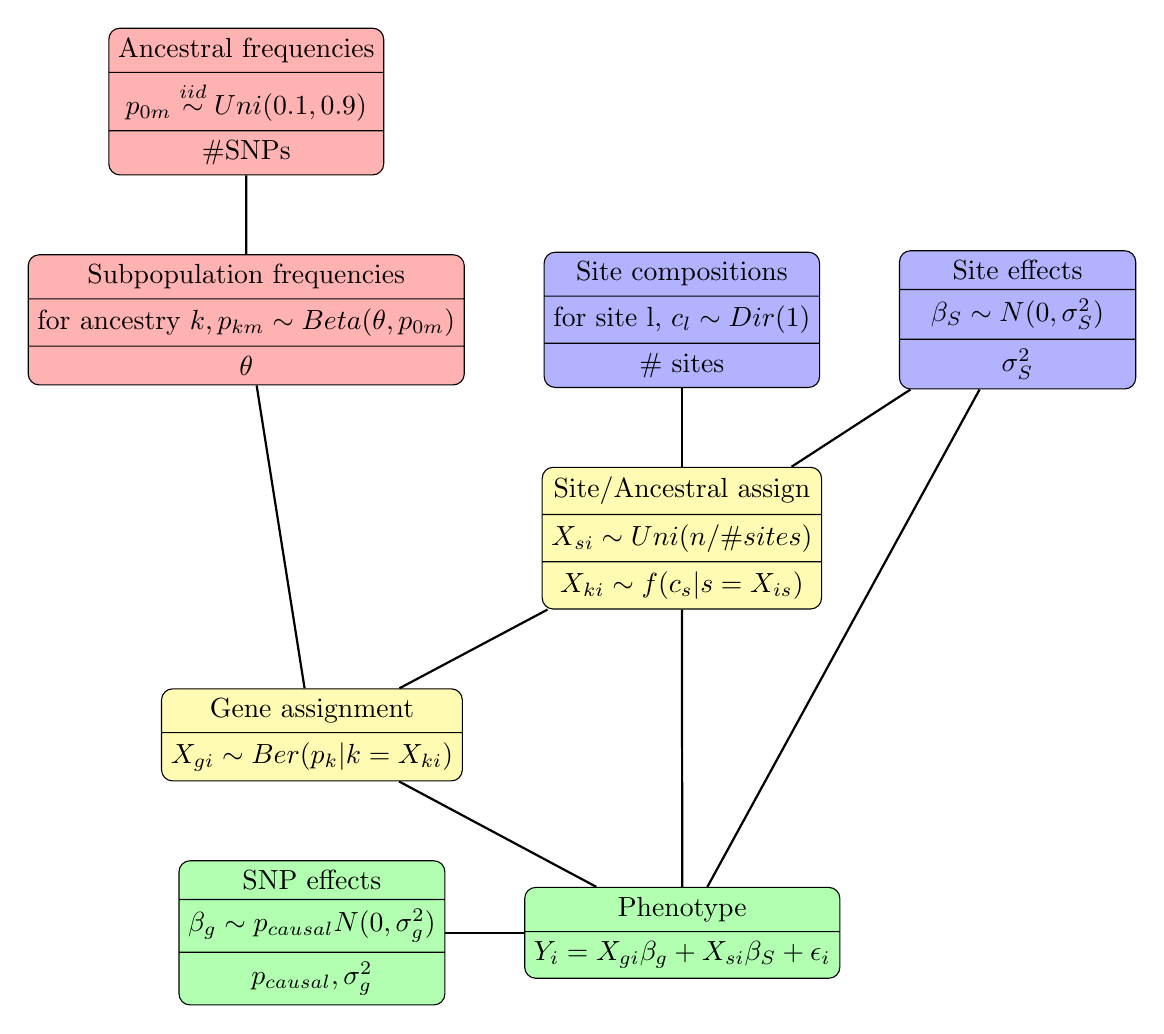
\begin{tikzpicture}[]
	
\node (anc_freq) [tnode, fill = red!30] {
  Ancestral frequencies
  \nodepart{second}
  $p_{0m} \stackrel{iid}{\sim} Uni(0.1, 0.9 $) 
  \nodepart{third}
  \#SNPs
};

  
\node (sub_freq) [tnode, fill = red!30, below=  of anc_freq] {
  Subpopulation frequencies
  \nodepart{second}
  for ancestry $k, p_{km} \sim Beta(\theta, p_{0m})$
  \nodepart{third}
  $\theta$ 
};



\node (site_comps) [tnode, fill = blue!30, right = of sub_freq] {
	Site compositions
	\nodepart{second}
	for site l, $c_l \sim Dir(1)$
	\nodepart{third}
  \# sites 
};         

\node (site_eff) [tnode, fill = blue!30, right = of site_comps] {
	Site effects
	\nodepart{second}
	$\beta_{S} \sim N(0,\sigma_S^2)$
	\nodepart{third}
	$\sigma_S^2$
};           

\node (site_anc_assign) [tnode, fill = yellow!30, below = of site_comps] {
	Site/Ancestral assign
	\nodepart{second}
	$X_{si} \sim Uni(n/\# sites)$
	\nodepart{third}
	$X_{ki} \sim f(c_s|s=X_{is})$
};           

\node (gene_assign) [dnode, fill = yellow!30, below left = of site_anc_assign] {
	Gene assignment
	\nodepart{second}
	$X_{gi} \sim Ber(p_k | k = X_{ki})$
	\nodepart{third}
};        

\node (gene_eff) [tnode, fill = green!30, below = of gene_assign] {
	SNP effects
	\nodepart{second}
	$\beta_{g} \sim p_{causal}N(0, \sigma_g^2)$
	\nodepart{third}
	$p_{causal}, \sigma_g^2$
};           

\node (pheno) [dnode, fill = green!30, right = of gene_eff] {
	Phenotype
	\nodepart{second}
	$Y_i = X_{gi}\beta_g + X_{si}\beta_S + \epsilon_i$
};           

   
\draw [arrow] (anc_freq) -- (sub_freq) -- (gene_assign);
\draw [arrow] (gene_eff) -- (pheno);
\draw [arrow] (site_comps) -- (site_anc_assign) ;
\draw [arrow] (site_eff) -- (site_anc_assign) -- (gene_assign) ;
\draw [arrow] (site_eff) -- (pheno) ;
\draw [arrow] (site_anc_assign) -- (pheno) ;
\draw [arrow] (gene_assign) -- (pheno) ;



           
\end{tikzpicture}



\begin{tikzpicture}

\end{tikzpicture}

\end{document}
